\section{Theoretical Analysis}
\label{analysis}

\paragraph{}
This theoretical analysis has, as its main purpose, showing how this circuit would behave in theory.

The values for the multiple components of the circuit can be found below:
\[ 
\left\{\begin{matrix}
	R_{1}= 1000 \Omega\\	
	R_{2}= 1000 \Omega\\
	R_{3}= 100000 \Omega\\
	R_{4}= 1000 \Omega\\
	C_{1}= 220 nF\\
	C_{2}= 220 nF\\
	C_{3}= 220 nF\\
	
\end{matrix}\right.
\]


\paragraph{}It is important to note that the following theoretical analysis is based upon the ideal OP-AMP model (and so, we are assuming that $Z_i = \infty$ and that $Z_o = 0$).

From here, by analysing the circuit, we can formulate the following system of equations:

\[ 
\left\{\begin{matrix}
	|Z_i| = |Z_{C_1} + R_1 \parallelsum \infty| = |Z_{C_1} + R_1|\\
	|Z_o| = |Z_{C_2} + \parallelsum (R_2 + R_3 \parallelsum 0)| = |Z_{C_2} \parallelsum R_2|\\
\end{matrix}\right.
\]

Besides this system, we can also derive the following system:

\[ 
\left\{\begin{matrix}
	v_- = v_+ = \frac{R_1}{R_1 + Z_{C_1}} v_i\\
	v_A = (1 + \frac{R_3}{R_4}) v_-\\
	v_o = \frac{Z_{C_2}}{Z_{C_2} + R_2} v_A
\end{matrix}\right.
\]

Finally, to calculate the central frequency, we need to calculate the average between the high cut-off frequency and the low cut-off frequency:

\[
\omega_{0}=\sqrt{\omega_{L} \times \omega_{H}}
\]


Considering that $Z_{C_1} = \frac{1}{j \omega C_1}$ and that $Z_{C_2} = \frac{1}{j \omega C_2}$, we can write the function used to determine the gain at the central frequency, that is given by:

\[
Gain = \displaystyle\left\lvert \frac{Z_{C_2}}{Z_{C_2}+R_2} \times (1+\frac{R_3}{R_4}) \times \frac{R_1}{R_1+Z_{C_1}} \right\rvert
\]

And, to obtain the gain in dB, we just need to:
\[
Gain (dB) = 20 \times \log_{10} (Gain)
\]

\paragraph{}And so, we were finally able to solve the circuit by simulation. The final results for this stage were obtained and are presented:

\begin{figure}[H] \centering
	\includegraphics[width=0.7\linewidth]{theo.eps}
	\caption{Theoretical frequency response - gain[dB]}
	\label{fig:gain_theo}
\end{figure}

\begin{figure}[H] \centering
	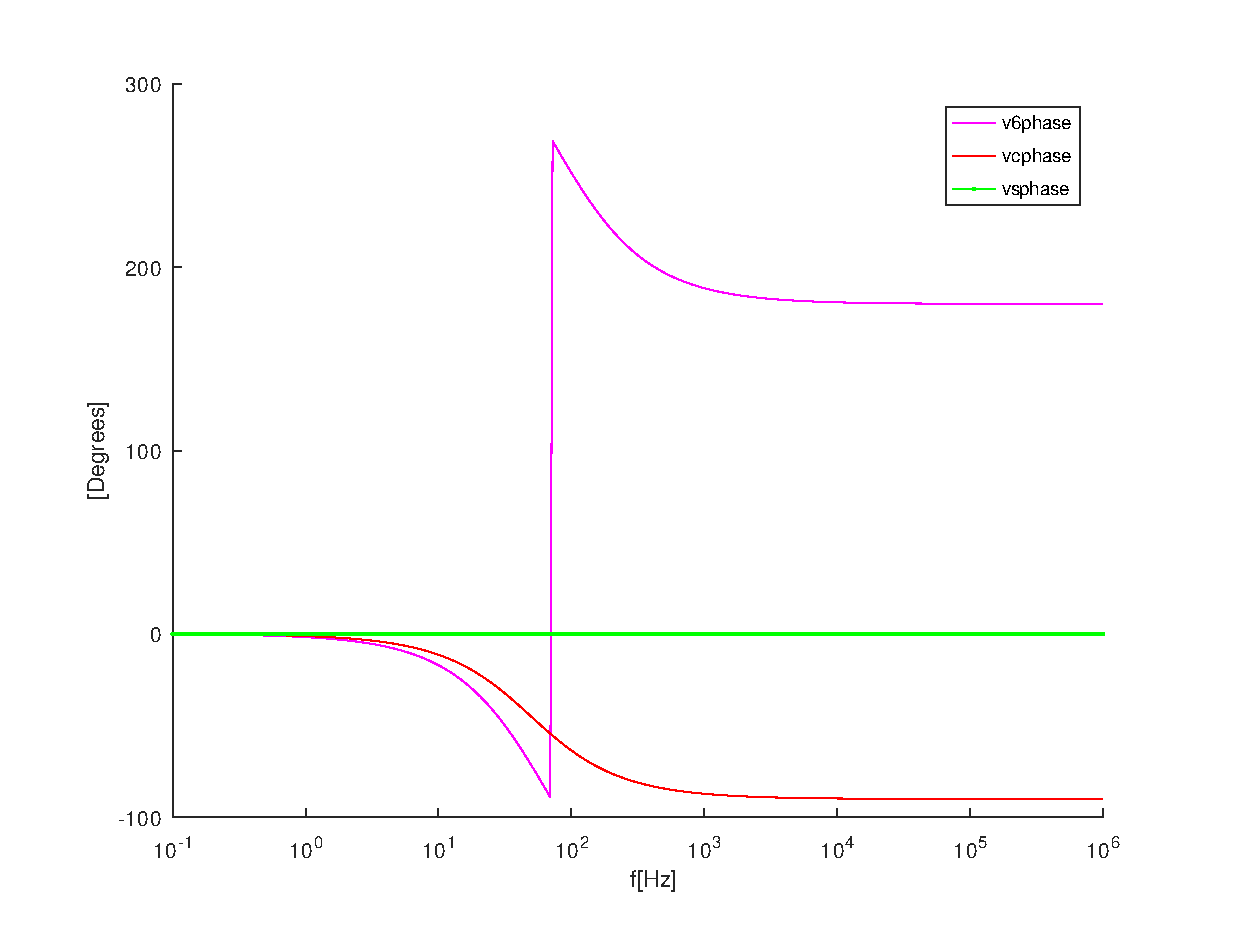
\includegraphics[width=0.7\linewidth]{phase.eps}
	\caption{Theoretical frequency response - phase[deg]}
	\label{fig:phase_theo}
\end{figure}

\begin{table}[H]
\centering
\begin{tabular}{|l|l|} 
\hline
\textbf{Characteristics} & \textbf{Values}  \\ \hline
Gain & 67.3177 V \\ \hline 
Gain dB & 36.5626 dB \\ \hline 
Gain Deviation & -3.4374 dB \\ \hline 
Lower Cut Off Frequency & 398.107 Hz \\ \hline 
Higher Cut Off Frequency & 2511.886 Hz \\ \hline 
Central Frequency & 1000.0 Hz \\ \hline 
Frequency Deviation & 0.0 Hz \\ \hline 
Bandwidth & 2113.779 Hz \\ \hline 
Input Impedance & 1234.242 Ohm \\ \hline 
Output Impedance & 822.637 Ohm \\ \hline 
\end{tabular}
\end{table}

\paragraph{}Analyzing the table above with detail, there are two specific values that are of great interest to this report: the central frequency and the gain at central frequency. When coming to the central frequency, the objective of obtaining a value of 1000 Hz was fulfilled. Looking now at the gain at central frequency, a value of  36.5626 dB was computed, while our objective was to compute a value of 40 dB. Even though the exact value was not obtained, the value we got is very similar to the desired one (with a deviation of -3.4374 dB, to be more precise), this way we can safely say the major objectives were successfully achieved.


